\section{Il codice}
Il videogioco ha parti di codice molto complesse,rendendo l'inclusione del codice irrealizzabile quindi cercherò di riassumere il processo con cui ho completato il progetto

\subsection{schermata menù}
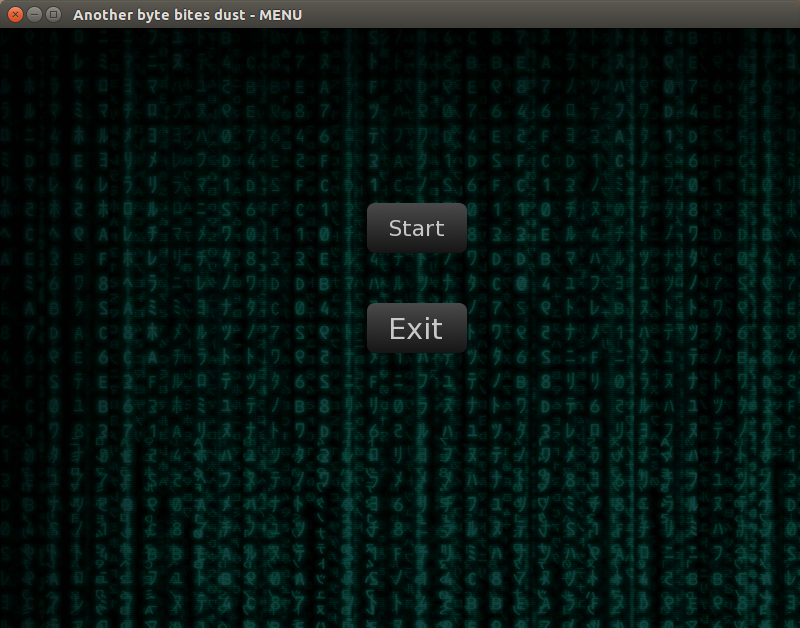
\includegraphics[scale=0.4]{menu.png}
La finestra è creata utilizzando la RenderWindow fornita da SFML.
Il menù contiene una form creata utilizza TGUI la quale contiene i due bottoni start e exit. La form contiene anche l'animazione in background che permette di cambiare sfondo ogni n secondi.
\subsection{Schermata gioco}
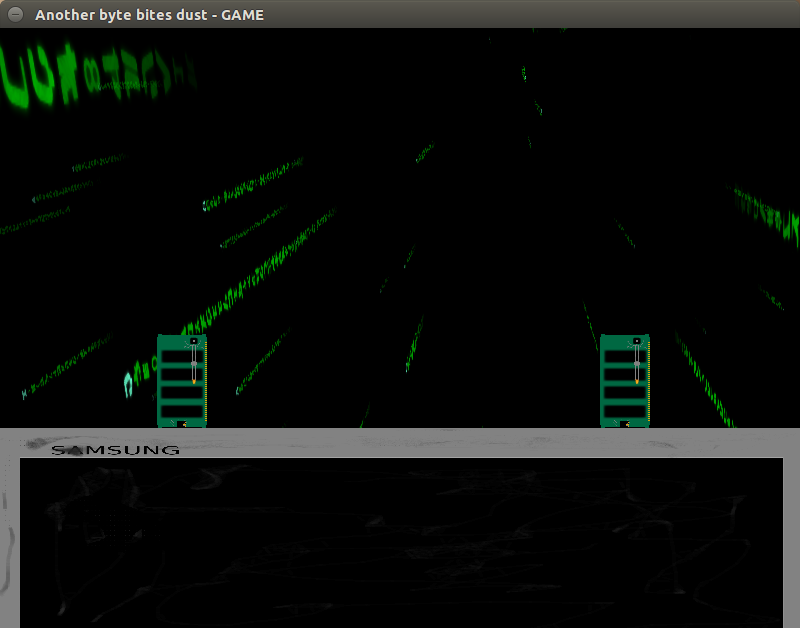
\includegraphics[scale=0.4]{game.png}
Premuto il tasto start la form viene eliminata e si inizializza ogni risorsa utilizzata nel gioco (textures,suoni,immagini).Al caricamento delle risorse il mondo sarà mostrato (monitor o terreno + galassia matrix o sfondo) e i due giocatori (due RAM) cadranno da metà finestra (per mostrare l'implementazione della gravità nel gioco. I due giocatori potranno, attraverso i tasti direzionali (freccie direzionali o WASD) muoversi nel mondo e saltare(sempre prendendo in considerazione la gravità). Al contatto dei due giocatori attraverso attacchi come il pugno o la caduta in volo, uno dei due perdere punti vita e con l'andare dei colpi perderà.
\section{Le difficoltà}
Per quanto il gioco sia teoricamente facile, la sua realizzazione pratica è stata abbastanza studiata.
\subsection{Le animazioni}
Per realizzare le animazioni il programmatore a più metodi a disposizione
\begin{itemize}
\item Creare una immagine(frame) per ogni parte del movimento
\item Creare una sola immagine(sprite) con uno scheletro ed utilizzare le matrici di trasformazione per modificare l'immagine
\item Creare un modello 3D con scheletro e considerare solo due dimensioni
\end{itemize}
La creazione di animazioni non è semplice poichè richiede molto tempo e/o software commerciali da centinaia di euro. La prima opzione si è rivelata la più economica. Ho creato una sprite del giocatore e, partendo da quella, tramite un programma di editing immagine, ho modificato gambe e braccia per n volte, creando una sensazione di movimento.
\subsection{La gestione delle risorse}
Caricare un'immagine è semplice, mentre ottimizzare i tempi di caricamento no. Tramite la libreria Thor ho create un gestore di risorse in grado di caricare delle spritesheet, ovvero una sola immagine contenente più sprite e le loro animazioni. In questo modo, le risorse possono essere condivise da ogni giocatore, senza essere duplicate e soprattutto, caricandole insieme rendono il lavoro della GPU meno pesante.
\subsection{La gravità}
Simulare un salto o una caduta è abbastanza semplice, simulare delle accelerazioni nello spazio e nel tempo un po' di meno. Per rendere il salto credibile bisogna utilizzare teoremi come il metodo di Eulero o l'algoritmo di Størmer-Verlet ed applicarlo al piano del gioco dove 0 non è il centro ma l'ordinata maggiore è l'altezza l'ordinata minore e origine in $\frac{larghezza}{2}$ $\frac{altezza}{2}$
La formula viene descritta nella sottosezione degli fps.
\subsection{La gestione degli fps}
Gli fps(Immagini mostrate dal monitor al secondo) molti meccanismi semplici in meccanismi più complessi: il movimento di un oggetto nel mondo deve essere direttamente proporzionale al tempo tra un frame ed il successivo, complicando le formule utilizzate sia per il movimento che per la gravità.
$posizione (x,y_{corrente})$	\\
$velocit\grave{a} (x, y_{gravit\grave{a}} + y_{impulsi})$\\
$y_{posizione} = y_{posizione} + (y_{velocit\grave{a}} \times \Delta{Secondi})$\\
$y_{velocit\grave{a}} = y_{velocit\grave{a}} + (y_{Accelerazione} \times \Delta{Secondi})$\\